% !TeX encoding = UTF-8
% !TeX spellcheck = es_ES
% !TeX root = DccPowerDistribution.tex

\documentclass{DccDiyTools}
\usepackage[spanish]{babel}


\title{Dcc Power Distribution}
\subtitle{Manual de Usuario}
\author{Daniel Vilas}
\date{Julio 2022}

\dbType{M}
\dbDate{22}
\dbCode{000}
\dbStatus{Draft}
\dbVersion{0.1}
\dbImage{images/front.png}

\begin{document}

\maketitle


\section{Introduccion}
Dcc Power Distribution es un modulo "DCC DiY Tools" que recoje la señal DCC y la utiliza como fuente de alimentacion para otros modulos de una maqueta. 
El objetivo de este modulo es proporcinar una interface DCC para que el usuario de este modulo tenga la señal DCC y energia para sus propios modulos.

Los modulos "DCC DiY Tools" son una serie de "Herramientas DCC Hazlo tu Mismo", pensadas para la gente con conocimiento de las placas Arduino y similares
puedan desarrollar sus porpios modulos sin tener que preocuparse de las complejidades y de los problemas comunes. Cualquiera que tenga un sketch corriendo
sobre una placa blanca de prototipo y quiera moverla a su maqueta se puede beneficiar de este modulo y asi no depender de un ordenador. 

Este modulo de distribucion de energia viene de la necesidad de controlar una serie de desvios con servomotores para hacer un moviento lento y para una 
maqueta no siempre tiene conectado un bus de +12V conectado. Pero no esta limitado a esto. Cualquier modulo que neceiste recibir alimentacion y señal DCC,
 en TTL, puede servirse de este dispositivo. Las caracteristicas generales de este modulo son:

\begin{itemize}
    \item \textbf{Multi Alimentacion}: Se puede alimentar por DCC o por un adaptador de Corriente Continua
    \item \textbf{Auto seleccion de Alimentacion}: En caso de conectar DCC y un adaptador, sin cambiar la configuracion se usara el adaptador.
    \item \textbf{Opciones de configuración}: Mediante Jumpers y pads soldables se puede lograr cierto grado de configuracion.
    \item \textbf{Multiples salidas} de voltaje:
    \begin{itemize}
        \item \textbf{VDrive}: lo mismo de de entrada, menos algunas perdidas por proteccion y auto-seleccion
        \item \textbf{5V}: obtenidos mediante un Buck Converter
        \item \textbf{3.3V}: Ajustados linealmente de los 5V
    \end{itemize}
    \item \textbf{Varias entradas} de voltaje:
    \begin{itemize}
        \item \textbf{DCC}: 12-20V y esta protegido ante los otros dos
        \item \textbf{Barrel Jack}: Centro positivo 12-20V, protegido con DCC y desprotegido con el terminal 
        \item \textbf{Terminal de Tornillos}: Conectado en paralelo con el jack.
    \end{itemize}
    \item Hasta \textbf{1A Corriente maxima}: por salida. Ver apartado de alimentacion.
    \item \textbf{Interface DCC opto-aislada}: incorporda y configurable.
    \item \textbf{Conectores standard}: y cambiables
    \begin{itemize}
        \item \textbf{JST XH} paso 2.54mm: DCC. 
        \item \textbf{806-KLDX-0202-A}: Conector Jack 2mm 
        \item \textbf{Terminal} paso 3mm: Terminales atornillables.
    \end{itemize} 
    \item \textbf{Open Software Hardware}: Este modulo se basa en diferentes diseños OSH y asi mismo se publica como OSH.
\end{itemize}

\subsection{Objetivos}
DccPowerDistribution es modulo cuyo objetivo principal dotar de alimentacion para otros modulos DiY
para facilitar el desarrollo de otros modulos por parte del usuario. Los objetivos del modulo son:
\begin{itemize}
    \item \textbf{Facilitar la toma de energia} al usuario objetivo, que es una persona que sepa
de arduino y quiera mover su circuito a su maqueta.   
    \item \textbf{Funcionar solo con un bus DCC}: Debe ser capaz de recoger la corriente desde el bus
DCC si no hay un bus de Corriente Continua(CC) disponible. Como por ejemplo en maquetas de pruebas
    \item \textbf{Usar un Bus CC}: para no sobrecargar el bus DCC sin ser necesario.
    \item \textbf{Ser robusto ante caidas DCC}: Ante un cortocircuito las centrales y los boosters 
paran de suministrar corriente DCC, por lo que el bus CC debe ser prioritario.
    \item \textbf{Facilitar el uso de DCC}: Para que el usuario tenga una señal DCC en TTL y usarla
con su placa.
\end{itemize}

\newpage
\section{Guia Rapida}
% !TeX encoding = UTF-8
% !TeX spellcheck = es_ES
% !TeX root = DccPowerDistribution.tex

Esta seccion es como empezar rapidamente con la configuracion por defecto, recomendamos leer todas las instrucciones para los diferentes
opciones de configuracion. 
\subsection{Soldaturas de los conectores}
El primer paso es escoger los conectores mas adecuados para nuestra maqueta, siendo la seccion de guia rapida, presuponemos que se utilizaran
los incluidos con el kit.

El segundo paso es soldar los conectores DCC, se suminstran unos JST XH 2.54, para dos y 4 vias. El de dos vias (J1) se usa para conectar a la señal DCC,
ya sea de la central o de un Booster. Mientras que J7, el conector de 4 vias, es la señal DCC
en TTL, valida para la libreria DCC de aurdino
\begin{figure}[h]
    \centering
    \begin{tikzpicture}
        \node[inner sep=0pt] (russell) at (0,0)
            {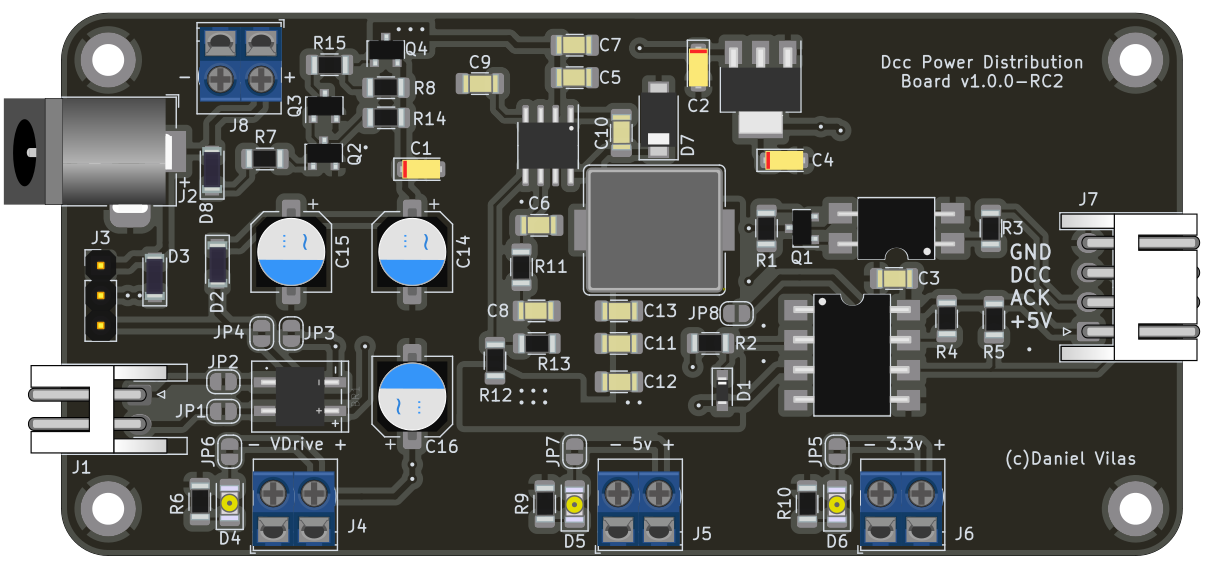
\includegraphics[scale=1.3]{images/front.png}};
        %\draw [very thin, green] (-6,-3) grid (6,3);
        \draw [color=red](-6.5,-0.7) rectangle (-4.5,-2.1); 
        \node [text width = 1cm] at (-7.1,-1.4){A la señal DCC};
        \draw [color=red](4.8,-1) rectangle (6.6,1.1);
        \node [text width = 1cm] at (7.2, 0.05){A un Decoder};
        %\node[below] {$a$};
    \end{tikzpicture}
    \caption{Conectores Dcc}
    \label{fig:DccConnectors}
\end{figure}

Los siguentes elementos a soldar, por tamaño, son los terminales para la salida de voltaje/corriente. 
En la guia rapida suponemos que se usan Los bloques terminales atornillables.

\begin{figure}[h]
    \centering
    \begin{tikzpicture}
        \begin{scope}
            \clip (-4.3,0) rectangle  (4.3,1.5);
            \node[inner sep=0pt] (russell) at (0.1,3)
                {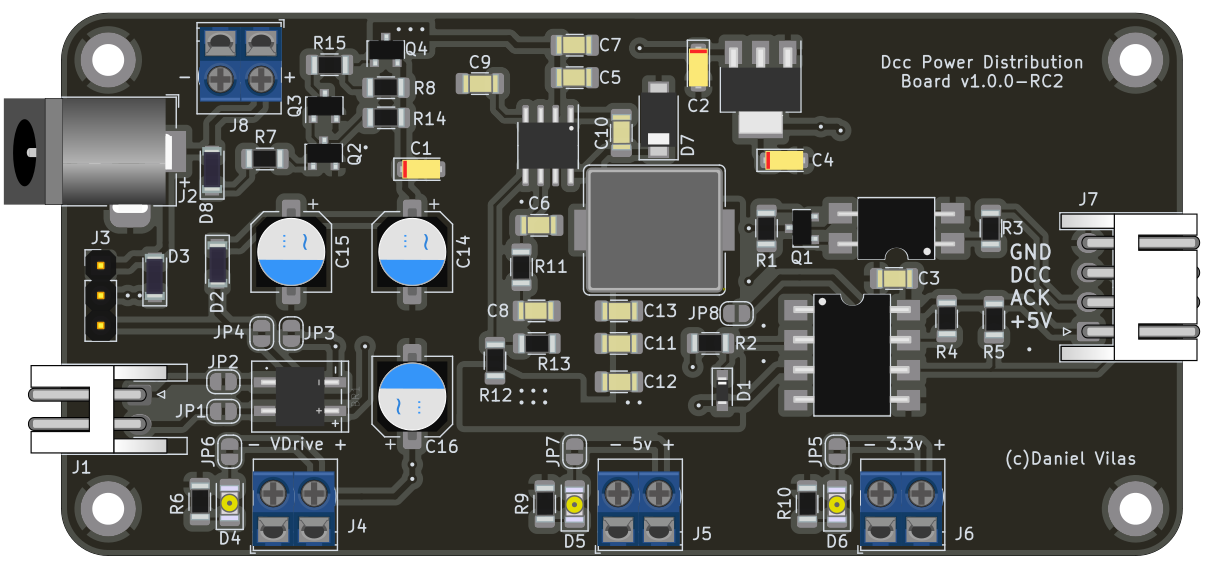
\includegraphics[scale=1.3]{images/front.png}};
        \end{scope}
        %\draw [very thin, green] (-5,-1) grid (5,2);
        \draw [color=red](-4,1.4) rectangle + (1.5,-1.6); 
        \node [text width = 1.3cm] at (-3.3,-0.5){VDrive};
        \draw [color=red](-0.2,1.4) rectangle + (1.5,-1.6); 
        \node [text width = 1.3cm] at (0.5,-0.5){+5V};
        \draw [color=red](2.7,1.4) rectangle + (1.5,-1.6); 
        \node [text width = 1.3cm] at (3.4,-0.5){+3.3V};
        %\node[below] {$a$};
    \end{tikzpicture}
    \caption{Salida Voltaje y Corriente}
    \label{fig:VccOutConnectors}
\end{figure}

Finalizaremos la soldadura añadiendo un solo conector de entrada, o bien el Jack o bien el terminal, segun lo que tengamos
disponible. Si vamos a usar un transformador con una jack (Centro positivo), soldaremos el Jack, pero si vamos a usar un
bus de corriente continua (dos cables) es mejor usar el terminal.

\begin{figure}[H]
    \centering
    \begin{minipage}{0.45\textwidth}
    \begin{tikzpicture}
        \centering
        \begin{scope}
            \clip (-2,-1.5) rectangle  +(4,2.9);
            %\draw [very thin, green, fill=yellow]  (-6,-3) rectangle (6,4);
            \node[inner sep=0pt] (russell) at (5,-1.9)
                {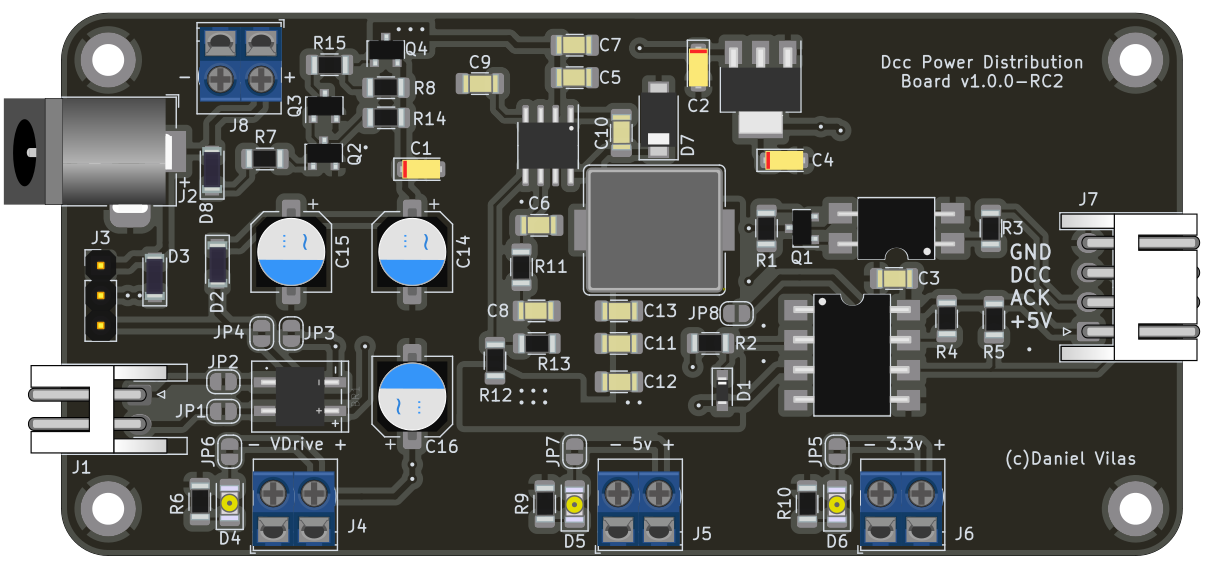
\includegraphics[scale=1.3]{images/front.png}};
            %\draw [very thin, green]  (-7,-3) grid (6,4);
        \end{scope}
        %\draw [very thin, green] (-3,-2) grid (3,2);
        \draw [color=red](-2,0.3) rectangle + (2.6,-1.6);
        \node [text width = 1.3cm] at (-2.5,-0.5){Jack 2mm};
    \end{tikzpicture}
    \caption{Entrada Voltaje Jack}
    \label{fig:VccInJack}
    \end{minipage}
    \hfill
    \begin{minipage}{0.45\textwidth}
    \centering
    \begin{tikzpicture}
        \begin{scope}
            \clip (-2,-1.5) rectangle  +(4,2.9);
            %\draw [very thin, green, fill=yellow]  (-6,-3) rectangle (6,4);
            \node[inner sep=0pt] (russell) at (5,-1.9)
                {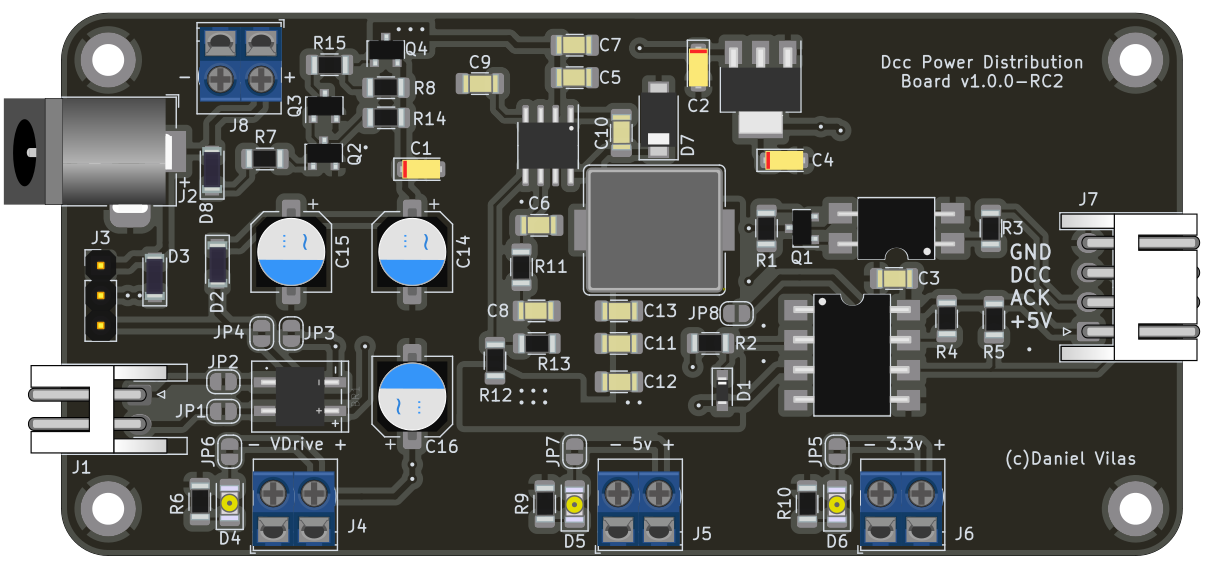
\includegraphics[scale=1.3]{images/front.png}};
            %\draw [very thin, green]  (-7,-3) grid (6,4);
        \end{scope}
        %\draw [very thin, green] (-3,-2) grid (3,2);
        \draw [color=red](0.2,-0.3) rectangle + (1.4,1.6);
        \node [text width = 1.3cm] at (1,2){Terminal Entrada};

    \end{tikzpicture}
    \caption{Entrada Voltaje Terminal}
    \label{fig:VccInTerminal}
    \end{minipage}
\end{figure}
Por ultimo como en cada proceso de soldadura, usar un tester para asegurarse antes de que no haya un cortocircuito
entre las soldaduras.
\subsection{Conexiones de entrada}
Con la maqueta apagada y el bus de alimentacion sin corriente, podremos procedera a conectar la entrada de alimentacion.
Tanto la señal DCC como la conexion a Corriente Continua. Para el conector DCC, hay que usar un cable terminado y 
crimpado con un Conector JST XH de dos vias, suministrado con el modulo, el otro exremo de este cable se debera conectar
a la central DCC o Booster como si fuera un tramo de via más.

\begin{figure}[H]
    \centering
    \begin{tikzpicture}
        \begin{scope}
            \clip (-1.5,-1) rectangle  + (3,2);
            %\draw [very thin, green, fill=yellow]  (-6,-3) rectangle (6,4);
            \node[inner sep=0pt] (russell) at (5.1,1.25)
                {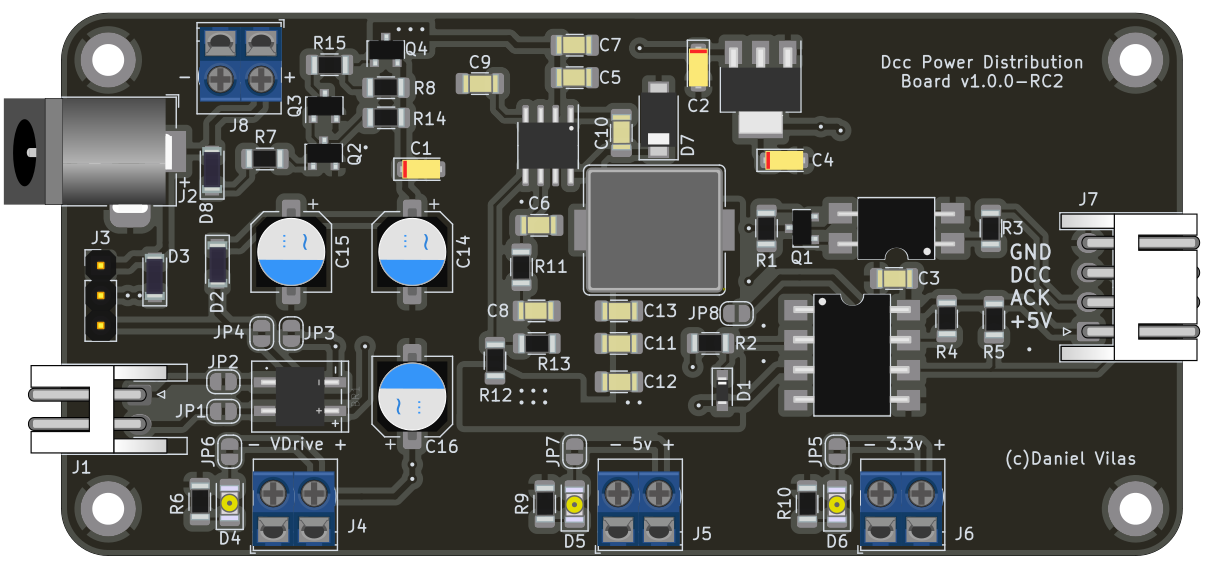
\includegraphics[scale=1.3]{images/front.png}};
            %\draw [very thin, green]  (-7,-3) grid (6,4);
        \end{scope}
        %\draw [very thin, green] (-3,-2) grid (3,2);
        \draw [color=red](-1.5,-0.9) rectangle + (2.3,1.5);
        \node [draw, text width = 2cm] at (-4,-0.15){Central o Booster};
        \draw [color=gray, line width=3pt,cap=round] (-2.9,0.06) -- (-1.4,0.06);
        \draw [color=lightgray, line width=3pt,cap=round] (-2.9,-0.25) -- (-1.4,-0.25);
    \end{tikzpicture}
    \caption{Entrada Señal DCC}
    \label{fig:DccIn}
\end{figure}
No es necesario una polaridad concreta, por lo que se pueden conectar a la via J o K indistintamente. No obstante se 
recomienda usar siempre la misma polaridad en todos los modulos iguales en la maqueta.

Si se va a usar un adaptador con un Jack 2mm, asegurarse de que sea centro positivo y conectarlo.
Pero en el caso de usar el terminal atornillable revisar la polaridad marcada en la placa con los simbolos + y -
\begin{figure}[H]
\centering
\begin{tikzpicture}
    \begin{scope}
        \clip (-1.5,-1) rectangle  +(3,2);
        %\draw [very thin, green, fill=yellow]  (-7,-3) rectangle (7,5);
        \node[inner sep=0pt] (russell) at (6.2,-3.55)
            {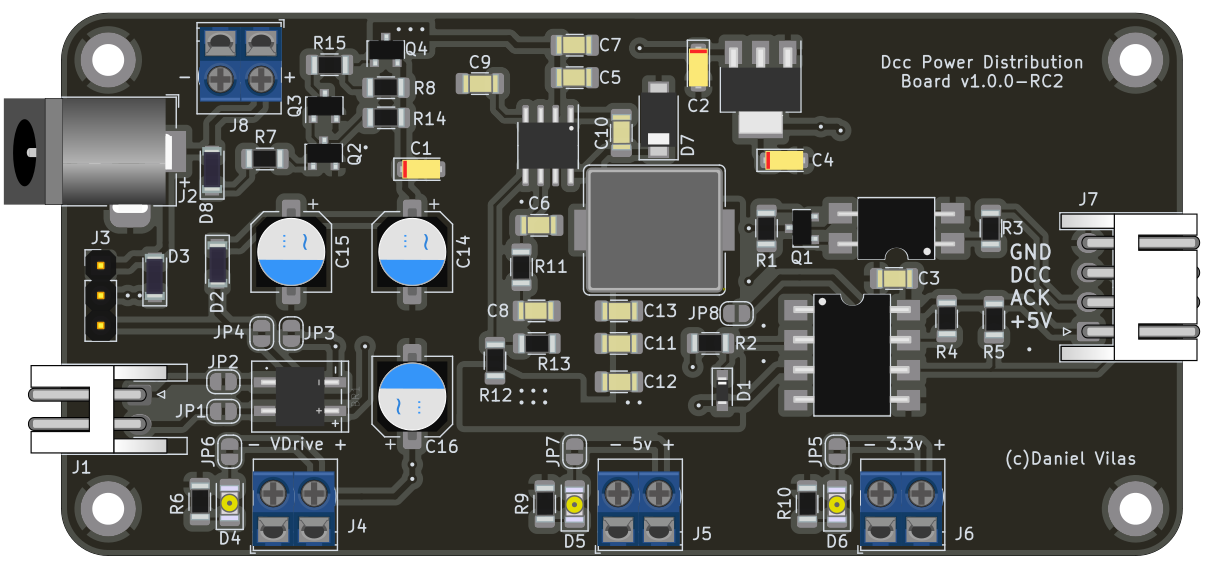
\includegraphics[scale=2]{images/front.png}};
        %\draw [very thin, green]  (-7,-3) grid (6,4);
    \end{scope}
    %\draw [very thin, green] (-3,-2) grid (3,2);
    \draw [color=red](-1.2,-0.8) rectangle + (2.2,2);
    \node [draw, text width = 1.7cm] at (-0.1,2.3){Adaptador CC};
    \draw [color=black, line width=3pt,cap=round] (-0.4,1.8) -- (-0.4,1.05);
    \draw [color=violet, line width=3pt,cap=round] (0.3,1.8) -- (0.3,1.05);
    \draw [color= yellow, line width=2pt] (-1,-0) circle[radius=0.3];
    \draw [color= yellow, line width=2pt] (.75,-0) circle[radius=0.3];
\end{tikzpicture}
\caption{Entrada Voltaje Terminal}
\label{fig:VccInTerminal2}
\end{figure}


Una vez conectado la alimentacion de entrada, podremos encender la maqueta y comprobar que todos los volajes
son correctos. Para ello se incluyen tres leds, uno para cada salida y se encenderan en cuanto haya voltaje
en dicha salida. Y ademas podremos medir con un polimetro
el voltaje entre los dos bornes del terminal.

\begin{figure}[h]
    \centering
    \begin{tikzpicture}
        \begin{scope}
            \clip (-4.3,0) rectangle  (4.3,1.5);
            \node[inner sep=0pt] (russell) at (0.1,3)
                {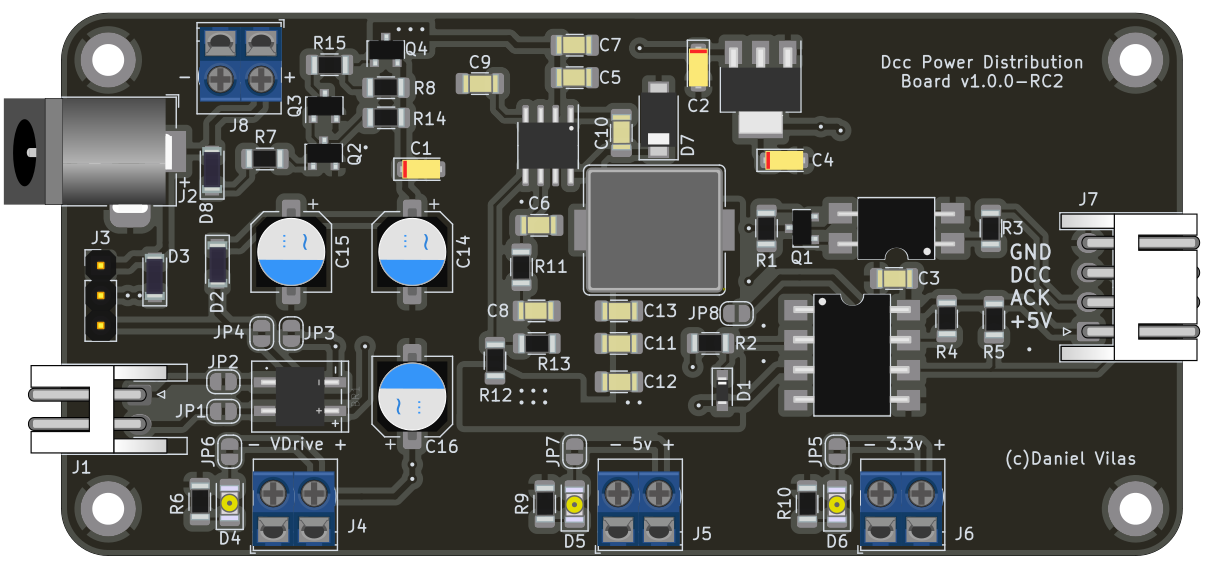
\includegraphics[scale=1.3]{images/front.png}};
        \end{scope}
        %\draw [very thin, green] (-5,-1) grid (5,2);
        \draw [color=red](-4,1.4) rectangle + (1.5,-1.6); 
        \node [text width = 1.3cm] at (-3.3,-0.5){VDrive};
        \draw [color=red](-0.2,1.4) rectangle + (1.5,-1.6); 
        \node [text width = 1.3cm] at (0.5,-0.5){+5V};
        \draw [color=red](2.7,1.4) rectangle + (1.5,-1.6); 
        \node [text width = 1.3cm] at (3.4,-0.5){+3.3V};
        \draw [color= yellow, line width=2pt] (-4.1,0.6) circle[radius=0.35];
        \draw [color= yellow, line width=2pt] (-0.3,0.6) circle[radius=0.35];
        \draw [color= yellow, line width=2pt] (2.6,0.6) circle[radius=0.35];
        %\node[below] {$a$};
    \end{tikzpicture}
    \caption{Salida Voltaje y Corriente}
    \label{fig:VccOutLeds}
\end{figure}

\subsection{Salida DCC}
Para conectar la alimentacion y las señales DCC a un Arduino, solo se necesita el conector JST XH de 4 vias. Para ello
se incluye un cable donde un estremo es JST XH y el otro son puntas macho Dupont sueltas. En la PCB esta marcado que señal
es cada cable.

\begin{figure}[H]
    \centering
    \begin{tikzpicture}
    \begin{scope}
        \clip (-2,-2) rectangle  + (4,4);
        %\draw [very thin, green, fill=yellow]  (-6,-4) rectangle (12,8);
        \node[inner sep=0pt] (russell) at (-8.1,0)
            {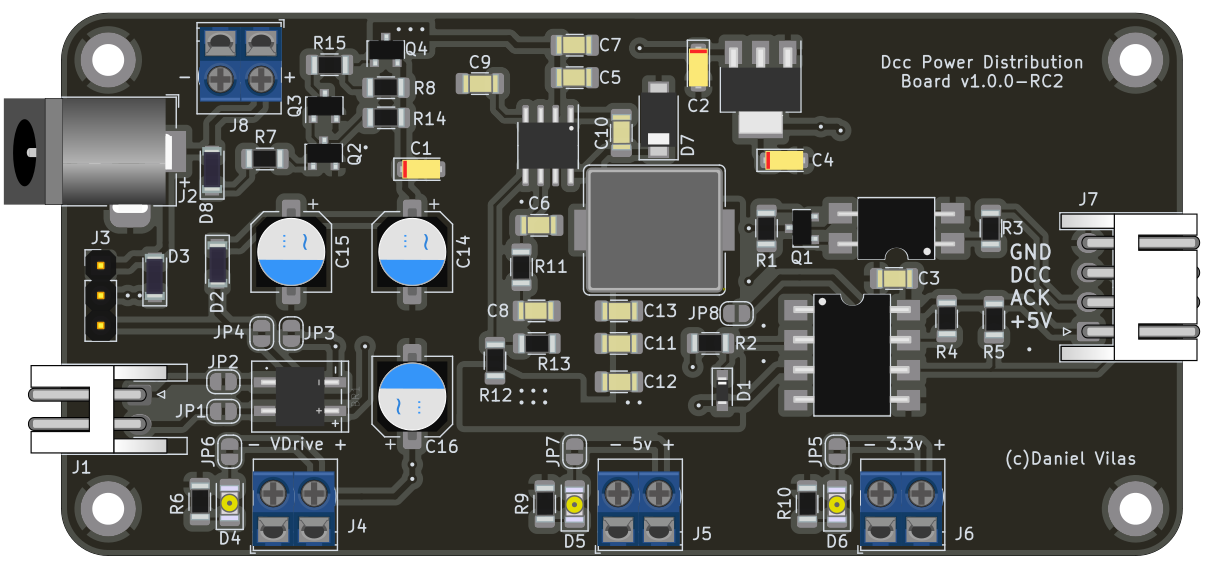
\includegraphics[scale=2]{images/front.png}};
        %\draw [very thin, green]  (-7,-3) grid (6,4);
    \end{scope}
    %\draw [very thin, green] (-3,-2) grid (3,2);
    \draw [color=yellow,line width=2pt](-1.6,-0.9) rectangle + (1.6,1.8);
    
    \node[right] at (4,1) {GND - A GND del aurdino};
    \node[right] at (4,0.33) {DCC - A Pin DCC (2)};
    \node[right] at (4,-0.33) {ACK - A Pin ACK (3)};
    \node[right] at (4,-1) {+5V - A 5V del Arduino)};
    
    \draw [color=black, line width=3pt,cap=round] (2.0,0.75) -- (4,1);
    \draw [color=blue, line width=3pt,cap=round] (2,0.25) -- (4,0.33);
    \draw [color=orange, line width=3pt,cap=round] (2,-0.25) -- (4,-0.33);
    \draw [color=red, line width=3pt,cap=round] (2.0,-0.75) -- (4,-1);
\end{tikzpicture}
    \caption{Entrada/Salida Señal DCC}
    \label{fig:DccOut}
\end{figure}
Por defecto la placa DCC Power Distribution esta configurada para que por la linea +5V
este conectada al bus de 5V de salida, por lo que se puede usar para alimentar un Arduino
sin problemas. Si el Arduino ya tiene su propia alimentacion, puede desconectarse este pin
o cambiar la configuracion de la placa. 

Los pines a los que conectar las señales DCC y ACK son 2 y 3 respectivamente para los
ejemplos de la libreria NmraDcc.

En este momento ya se puede encender la maqueta y usar el Arduino como decoder DCC.

\subsection{Otras salidas de Voltaje}
DCC Power Distribution incluye otras tres salidas de voltaje, a las que se pueden conectar
otros dispositivos, para ello solo hay que instalar los cables y respetar la polaridad
marcada con los simbolos + y -.

\begin{figure}[h]
    \centering
    \begin{tikzpicture}[scale=1]
        \begin{scope}
            \clip (-6.5,0) rectangle  +(13,2.5);
            \node[inner sep=0pt] (russell) at (0.1,4.75)
                {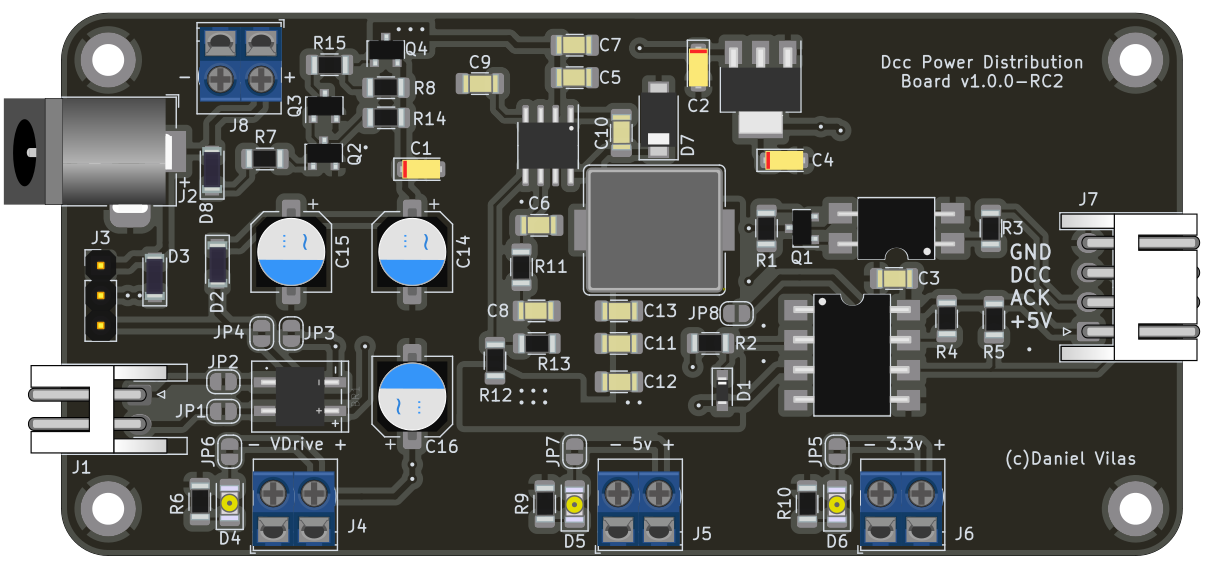
\includegraphics[scale=2]{images/front.png}};
        \end{scope}
        
        \draw [color=red](-6.2,2.4) rectangle + (2.3,-2.5); 
        \node [text width = 1.3cm] at (-5,-0.5){VDrive};
        \draw [color=red](-0.3,2.4) rectangle + (2.3,-2.5); 
        \node [text width = 1.3cm] at (1,-0.5){+5V};
        \draw [color=red](4.1,2.4) rectangle + (2.3,-2.5); 
        \node [text width = 1.3cm] at (5.4,-0.5){+3.3V};
        \draw [color= yellow, line width=2pt] (-4.45,2.05) circle[radius=0.3];
        \draw [color= yellow, line width=2pt] (-5.95,2.05) circle[radius=0.3];
        \draw [color= yellow, line width=2pt] (0.2,2.05) circle[radius=0.3];
        \draw [color= yellow, line width=2pt] (1.1,2.05) circle[radius=0.3];
        \draw [color= yellow, line width=2pt] (4.5,2.05) circle[radius=0.3];
        \draw [color= yellow, line width=2pt] (5.65,2.05) circle[radius=0.3];
    \end{tikzpicture}
    \caption{Salida Voltaje y Corriente}
    \label{fig:VccOutConnectors2}
\end{figure}


\newpage
\section{Caracteristicas Tecnicas}
% !TeX encoding = UTF-8
% !TeX spellcheck = es_ES
% !TeX root = DccPowerDistribution.tex
\subsection{Objetivos}
Como se ha dicho DccPowerDistribution es modulo cuyo objetivo principal dotar de alimentacion para otros modulos DiY
para facilitar el desarrollo de otros modulos por parte del usuario. Los objetivos tecnicos del modulo son:
\begin{itemize}
    \item \textbf{Autoseleccion DCC - CC} Cuado esten los dos buses conectados debe usar Corriente Continua.
sin que el usuario tenga que cambiar interruptores.    
    \item \textbf{1A Corriente} continua: que permita mover un motor y algunos accesorios
sin problemas
    \item \textbf{1.5A Corriente} maximo. Como margen de seguridad.
    \item \textbf{Tres salidas de Voltaje}:
    \begin{itemize}
        \item \textbf{VDrive}: El Voltaje de entrada para alimentar otros modulos.
        \item \textbf{+5V}: 5 Voltios para arduinos y otros componentes
        \item \textbf{+3.3V} 3.3 Voltios para los nuevos Arduinos ARM y otros microcontroladores similares
    \end{itemize} 
\end{itemize}

\subsection{Diagrama de Bloques}
El diseño del modulo en bloques es el siguiente:
\begin{figure}[H]
    \centering
    \begin{tikzpicture}
    %\draw [very thin, green] (-1,-3) grid (12,4);
    \begin{scope}[shift={(0,2)}]
        \node [left] (txtCcB) at (0, 1){CC Bloque};
        \pic(picCcB)[rotate=-90] at (1,1)  {screwTerminal} ;
        \node [left](txtCcJ) at (0, 0){CC Jack};
        \pic (picCcJ) at (1,0)  {jack} ;

        \draw[] (txtCcB.east) -- (picCcB-cable-down.center);
        \draw[] (txtCcJ.east) -- (picCcJ-cable.center);
        \node[draw](proteccion) at (4,0.5) {Protección};

        \draw[] (picCcB-cable-up.center) -- (2.25,1) 
            -- (2.25, 0.5) -- (proteccion.west);
        \draw[] (picCcJ-point.center) -- (2.25,0)
            -- (2.25, 0.5);
        \node[](ptVDrive)  at (proteccion.east-| 6,0) {};
        \node[above](lblVdrive) at (ptVDrive.center)  {VDrive};
        \draw (proteccion.east) -- (ptVDrive.center);
        \draw (2.75, 0.5) -- (2.75,1.25) -- (5.25,1.25) 
            -- (5.25,0.5);
        \pic[] at (proteccion.center |- 0,1.25) {SmallDiode};
        \draw[blue, dashed] (3.5,1.25) -- (3.5,1.5) -- (4.5,1.5)
            -- (4.5,1.25);
        \draw[blue, dashed] (proteccion.center |- 0,0)
            -- (5.25,0) -- (5.25,.5);
    \end{scope}

    \begin{scope}
        \node [left] (txtDccIn) at (0, 0){DCC};
        \pic[rotate=-90] (picDccIn) at(1,0){JstXh2};
        \pic[](DccDiode) at (3,0){DiodeBrigde};

        \draw[] (txtDccIn.east) -- (picDccIn-cable.center);
        \draw[] (picDccIn-pcb.center) -- (DccDiode-ac.center);

        \draw[] (DccDiode-cc.center) -- (DccDiode-cc.center -| proteccion.south)
            -- (proteccion.south);
    \end{scope}

    \begin{scope}[shift={(ptVDrive.center |- 0,0)}]
        \pic[](picOutVdrive)  at (0,0){screwTerminal};
        \node[below](lblOutVdrive)  at (picOutVdrive-cable-down.center){Vdrive};
        \draw[] (ptVDrive.center) -- (picOutVdrive-cable-up.center);
        \pic[rotate=-90,yscale=-1](picLedVdrive)  at (-0.75,0){SmallLed=green};
        \draw (0,0.5) -- (picLedVdrive-p.center |- 0,0.5) -- (picLedVdrive-p.center);
        \node[red, scale=.75]at(-0.4,0.5){X};
    \end{scope}

    \begin{scope}[shift={(ptVDrive.center -| 7.5,0)}]
        \node[draw](buck) at (0,0) {Buck}; 
        
        \node[](pt5V)  at (1.5,0) {};
        \node[above](lbl5V) at (pt5V.center)  {+5V};
        \draw (buck.east) -- (pt5V.center);
        \draw (ptVDrive.center) -- (buck.west);
    \end{scope}

    \begin{scope}[shift={(pt5V.center |- 0,0)}]
        \pic[](picOut5V)  at (0,0){screwTerminal};
        \node[below](lblOut5)  at (picOut5V-cable-down.center){+5V};
        \draw[] (pt5V.center) -- (picOut5V-cable-up.center);
        \pic[rotate=-90,yscale=-1](picLed5V)  at (-0.75,0){SmallLed=green};
        \draw (0,0.5) -- (picLed5V-p.center |- 0,0.5) -- (picLed5V-p.center);
        \node[red, scale=.75]at(-0.4,0.5){X};
    \end{scope}


    \begin{scope}[shift={(pt5V.center -| 10.5,0)}]
        \node[draw](ldo) at (0,0) {LDO};  
        \node[](pt33V)  at (1.5,0) {};
        \node[above](lbl33V) at (pt33V.center)  {+3.3V};
        \draw (ldo.east) -- (pt33V.center);
        \draw (pt5V.center) -- (ldo.west);
    \end{scope}

    \begin{scope}[shift={(pt33V.center |- 0,0)}]
        \pic[](picOut33V)  at (0,0){screwTerminal};
        \node[below](lblOut33)  at (picOut33V-cable-down.center){+3.3V};
        \draw[] (pt33V.center) -- (picOut33V-cable-up.center);
        \pic[rotate=-90,yscale=-1](picLed33V)  at (-0.75,0){SmallLed=green};
        \draw (0,0.5) -- (picLed33V-p.center |- 0,0.5) -- (picLed33V-p.center);
        \node[red, scale=.75]at(-0.4,0.5){X};
    \end{scope}

    \begin{scope}[shift={(lblVdrive.center |- 3,-2)}]
        \pic[](dccIface)at (0,0){DccIface};
        
    \end{scope}
    \draw[] (picDccIn-pcb.center -| 1.9,0) -- (1.9,0 |- dccIface-west-out.center) 
        -- (dccIface-west-out.center);
        \draw[] (4,0) -- (4,0 |- dccIface-west-in.center) 
        -- (dccIface-west-in.center);


    \begin{scope}[shift={(lbl5V.center |- dccIface-west.center)}]
        \pic[rotate=90](dccOut)at (0,0){JstXh4};

        \node[right](lblDccOutGnd) at (1,0.6) {GND};
        \node[right](lblDccOut) at (1,0.2) {DCC-TTL};
        \node[right](lblDccOutACK) at (1,-0.2) {DCC-ACK};
        \node[right](lblDccOut5V) at (1,-0.6) {+5V};
        
        \draw[red] (dccOut-c0.center) -- (lblDccOut5V.west);
        \draw[orange] (dccOut-c1.center) -- (lblDccOutACK.west);
        \draw[blue] (dccOut-c2.center) -- (lblDccOut.west);
        \draw[black] (dccOut-c3.center) -- (lblDccOutGnd.west);


        \draw (dccIface-east-out.center) -- (dccOut-p2.center);
        \draw (dccIface-east-in.center) -- (dccOut-p1.center);
        \draw (dccIface-east.center |- dccOut-p0.center) -- (dccOut-p0.center);
    \end{scope}

    \draw[] (pt5V.center |- 0,1.5) -- +(-1.2,0) -- +(-1.2,-3.3) arc(90:-90:.05)
    -- +(0,-.2)  arc(90:-90:.05) -- +(0,-.25);

    \node[red, scale=.75]at(8.4,1.5){X};
    \node[red, scale=.75]at(2.1,0){X};
    \node[red, scale=.75, rotate=90]at(4,1.5){X};
    
\end{tikzpicture}
    \caption{Diseño por Diagrama de Bloques}
    \label{fig:BlockDiagrama}
\end{figure}
Mediante jumpers y soldaduras es posible configurar la placa para alterar su funcionamiento.
Las lineas discontinuas azules son jumpers para poder hacer derivaciones (por defecto abiertos) y
las cruzes rojas son pistas para romper con puntos de soldaura cercanos para unir soldando.

\subsubsection{Seleccion de corriente}
La señal \textbf{DCC} va directa la \textbf{interface DCC} y a un puente rectificador
\textbf{AC -> CC} para poder ser usado como fuente de corriente, pero antes debe pasar
por el bloque \textbf{Proteccion}. 

Pero la prioridad es utilizar la corriente que venga de un adaptador Corriente Continua (CC), 
ya sea por el \textbf{Jack CC} o por el \textbf{Bloque CC} atornillable. 
Por lo que si hay corriente de una adaptador CC, el bloque \textbf{Proteccion} bloqueara la corriente
proveniente de la señal DCC y la linea \textbf{VDrive} sera alimentada desde el adaptador
pasando por diodo de proteccion en caso de tener corriente DCC y CC a la vez.

Es posbile evitar la proteccion con el jumper de bypass (lineas azules cerca del bloque) y
con los cortes (cruces rojas) cerca del retificador. Mirar el apartado de configuración para
más informacion.

Los dos conectores, \textbf{Jack CC} y \textbf{Bloque CC} atornillable, estan conectados
en paralelo directo, por lo que se debe tener cuidado en caso de conectar los dos.

\subsubsection{Distribucion de corriente}
Este modulo genera tres carriles de potencia, \textbf{VDrive}, \textbf{+5V} y \textbf{+3.3V}.
VDrive es tal cual la fuente que se ha selecionado y el resto se generan a partir de esta.

Los tres carriles acaban en un bloque terminal atornillable para conectar a otros modulos.
Junto al cual se haya un led para visualizar que existe dicho carril. Este led puede ser
inhibido, cortando una pista. Mirar el apartado de configuración para
más informacion.

El carril de 5 Voltios se crea mediante un circuito \textbf{Buck StepDown} generado con la herramienta
de diseño "WEBENCH Power Designer", siendo este más o menos el circuito de referencia del chip usado.

Asi mismo el carril de 3.3 Voltios se genera con un regulador lineal siguiendo el cortocircuito
de referencia del mismo.

\subsubsection{Interface DCC}
La interface DCC se basa en el diseño de referencia con dos optoaisladores, de tal forma que la
señal DCC se convierte en TTL y la linea ACK activa una carga en la red DCC.

El conector DCC incluye los siguientes puntos:
\begin{itemize}
    \item \textbf{+5V}: linea para TTL Alto, se utiliza de vuelta en el pin DCC-TTL. Puede ser configurada
para usar el rail \textbf{+5V}.
    \item \textbf{DCC-ACK}: un 1 logico aqui provacara que se active una carga en la red DCC
notificando un OK a la central (como una programacion correcta).
    \item \textbf{DCC-TTL}: Linea que repite la señal DCC en un valor valido TTL, usando como valor
la señal +5V del conector.
    \item \textbf{GND}: Nivel base GND para unir a otros modulos.
\end{itemize} 

\subsection{Limites}
DccPowerDistribution soporta varios Voltajes y corrientes maximas segun cual sea el conector que
se use y como se configuren los bypass. Los componentes se han elegido pensando en un consumo maximo
continuado de \textbf{1A}. Por especificaciones los elementos pueden soportar de manera continudada al
menos un 50\% más. 

La tablas siguente recogen los Voltajes aceptados recomendados, maximo sin bypass y maximo si activamos
el bypass para evitar la proteccion.

\begin{table}[H]
    \centering
    \renewcommand\theadfont{\bfseries}
    \setlength{\tabcolsep}{10pt}
    \renewcommand{\arraystretch}{1.5}
    \begin{tabular}{c |c |c |c |c |}
        entrada & \thead[b]{item} & \thead[b]{Recomendado} & \thead[b]{Maximo} & \thead[b]{Con Bypass} \\ 
        \Xhline{5\arrayrulewidth}
%Entrada DCC
        \rowcolor{Melon!15}
        & Voltaje &14-20V & \multicolumn{2}{c|}{12-24V} \\
        \cline{2 - 5}
        \rowcolor{Melon!10} \cellcolor{Melon!15}
        \multirow{-2}{*}{DCC}&Corriente & 1A & 1.5A & 2A \\ \Xhline{3\arrayrulewidth}
%Entrada Jack
        \rowcolor{blue!15} & Voltaje & 12-20V & \multicolumn{2}{c|}{10-24V} \\
        \cline{2 - 5}
        \rowcolor{blue!10} \cellcolor{blue!15} \multirow{-2}{*}{ \makecell{ \cellcolor{blue!15} Jack\\ \cellcolor{blue!15} Terminal}} & Corriente & 1A & 1.5A & 3A \\
        \Xhline{5\arrayrulewidth}
    \end{tabular}
    \caption{Limites de entrada}
    \label{tab:limiteEntrada}
\end{table}

\begin{table}[H]
    \centering
    \renewcommand\theadfont{\bfseries}
    \setlength{\tabcolsep}{10pt}
    \renewcommand{\arraystretch}{1.5}
    \begin{tabular}{c |c |c |c |c |}
        Salidas & \thead[b]{item} & \thead[b]{Recomendado} & \thead[b]{Maximo} & \thead[b]{Con Bypass} \\ 
        \Xhline{5\arrayrulewidth}
%Salida Vdrive        
        \rowcolor{BlueGreen!15}& Voltaje & \multicolumn{3}{c|}{Mismo que la entrada - 1.0V} \\
        \cline{2-5}
        \rowcolor{BlueGreen!10} \cellcolor{BlueGreen!15}
        \multirow{-2}{*}{Vdrive}&Corriente* & 1A & 1.5A & 3A \\ \Xhline{3\arrayrulewidth}
%Salida +5V        
        \rowcolor{red!15}& Voltaje & \multicolumn{3}{c|}{5V +/- 2\% con ruido} \\
        \cline{2-5}
        \rowcolor{red!10} \cellcolor{red!15}
        \multirow{-2}{*}{+5V}&Corriente* & 1A & 1.5A & 3A \\ \Xhline{3\arrayrulewidth}
%Salida +3.3V                
        \rowcolor{Goldenrod!15}& Voltaje & \multicolumn{3}{c|}{3.3V +/- 0.6\%} \\
        \cline{2-5}
        \rowcolor{Goldenrod!10} \cellcolor{Goldenrod!15}
        \multirow{-2}{*}{+3.3V}&Corriente* & 0.5A & 1A & 1A \\ \Xhline{3\arrayrulewidth}
   \end{tabular}
   \caption{Limites de salida}
   \label{tab:limiteSalida}
   \textbf{*}:La suma de la corriente de salidas no puede exceder el limite de corriente de entrada
\end{table}

DccPowerDistribution ha sido diseñado y probado para poder utilizar hasta 1A en total y lo componentes
escogidos para que segun sus especificaciones puedan soportar al menos 1.5A
\section{Configuracion}
\subsection{Objetivos de este documento}
\subsubitem{Otra}

% \begin{tip}{Test}
% Ejemplo de tip
% \end{tip}
\end{document}